\chapter{Združené rozdelenie pravdepodobnosti}\label{sec:joint_dist}

V predchádzajúcich kapitolách sme sa zaoberali modelovaním rozdelenia pravdepodobnosti jednotlivých náhodných premenných alebo cieľových premenných v kontexte regresie a klasifikácie. V oboch týchto prístupoch sme vychádzali prevažne z predpokladu, že modelujeme samostatnú premennú alebo závislosť jednej výstupnej premennej na vstupe. V praxi však častokrát pracujeme s viacerými náhodnými premennými súčasne, ktorých správanie môže byť navzájom ovplyvňované. Ich spoločné správanie popisuje tzv. \textit{združené rozdelenie pravdepodobnosti}.

Ak premenné modelujeme ako komponenty náhodného vektora, napríklad $\vec{X} = (X_1, X_2)$, potom znalosť ich združeného rozdelenia nám umožňuje odvodiť ďalšie dôležité vlastnosti systému – napríklad ako vyzerajú podmienené rozdelenia, marginálne rozdelenia alebo podmienená stredná hodnota jednej premennej vzhľadom k iným premenným. Tieto pojmy sú kľúčové nielen pre štatistické modelovanie ako také, ale aj pre praktické aplikácie ako sú predikcie, rozhodovania sa založené na týchto predikciách alebo celková analýza závislostí.

Presné vyjadrenie alebo odhad združeného rozdelenia je však zložitý, čo je podnecované vyšším počtom premenných. S rastúcim rozmerom vektora náhodných premenných rastie aj počet parametrov a miera závislosti, ktorú je potrebné zohľadniť. Preto sa častokrát používajú zjednodušujúce predpoklady, napríklad o nezávislosti alebo naopak špecifickej štruktúre závislosti medzi premennými.

V tejto kapitole sa zameriame na:
\begin{itemize}
  \item základy modelovania združených rozdelení, vrátane podmienených a marginálnych funkcií,
  \item rozklad združeného rozdelenia na marginálne rozdelenia a kopulovú funkciu,
  \item praktické aspekty odhadu združeného rozdelenia na základe údajov.
\end{itemize}

Konkrétne budeme v tejto kapitole pracovať so združenými rozdeleniami náhodných premenných rovnakého typu – teda buď čisto spojitými, alebo čisto diskrétnymi. Budeme rozoberať všeobecné princípy modelovania, analýzy a odhady takýchto rozdelení. Praktické príklady budú vychádzať z regresných a klasifikačných kontextov, kde sa využívajú znalosti o marginálnych a podmienených rozdeleniach. Pre ilustráciu štruktúry dát a závislostí medzi premennými využijeme nástroje popisnej štatistiky a vizualizačné techniky, ktoré sú súčasťou výstupov mnou implementovanej interaktívnej aplikácie. Táto aplikácia predstavuje aplikačnú časť tejto bakalárskej práce a poskytuje praktické vizualizačné a analytické nástroje na skúmanie združených rozdelení pravdepodobnosti, ktoré sú využité aj pri prezentácii výsledkov v tejto kapitole. Modelovanie zmesi spojitých a diskrétnych náhodných premenných, ako špecifický prípad heterogénnych štruktúr, bude predmetom samostatnej kapitoly, keďže ide o hlavnú problematiku, na ktorú sa v tejto práci chceme zamerať.


\section{Základy modelovania}\label{sec:joint_zaklady_modelovania}

\subsection{Funkčná reprezentácia}\label{subsec:joint_representation}

Podobne ako to bolo v jednorozmernom prípade, aj viacrozmerné združené rozdelenie možno reprezentovať rôznymi funkciami. My sa v tejto práci budeme zaoberať iba dvojrozmerným prípadom. Dve náhodné premenné $X_1$ a $X_2$ teda môžeme opísať buď pomocou ich spoločnej distribučnej funkcie (angl. joint cumulative distribution function – CDF), alebo pomocou ďalších vhodných nástrojov v závislosti od typu premenných.

\subsubsection{Kumulatívna distribučná funkcia (CDF)}\label{subsec:joint_cdf}

Spoločná distribučná funkcia $F(x_1, x_2)$ dvoch náhodných premenných $X_1$ a $X_2$ vyjadruje pravdepodobnosť, že obe premenné nadobudnú súčasne hodnoty najviac $x_1$ a $x_2$:

\begin{equation}
F(x_1, x_2) = \mathrm{Pr}(X_1 \leq x_1,\ X_2 \leq x_2),
\end{equation}

pričom vo vzťahu k združenej hustote týchto premenných platia nasledujúce vzťahy:

\begin{equation}
F(x_1, x_2) = \int_{-\infty}^{x_1} \int_{-\infty}^{x_2} f(y_1, y_2) \, dy_1 dy_2
\end{equation}

\begin{equation}
f(x) = \left. \frac{\partial^2 F(y_1, y_2)}{\partial y_1 \partial y_2} \right|_{y = x}
\end{equation}

\subsubsection{Združená hustota pravdepodobnosti (PDF)}\label{subsec:joint_pdf}

Ak sú premenné spojité, spoločné rozdelenie opisujeme prostredníctvom \textit{združenej hustoty pravdepodobnosti} (angl. joint probability density function – PDF) $f(x_1, x_2)$, ktorá udáva pravdepodobnostnú hustotu výskytu dvojice hodnôt v danej oblasti roviny $\mathbb{R}^2$.

V prípade diskrétnych premenných sa namiesto hustoty používa \textit{združená pravdepodobnostná funkcia} (angl. joint probability mass function – PMF), ktorá každému páru hodnôt $(x_1, x_2)$ priraďuje konkrétnu pravdepodobnosť výskytu: 

\begin{equation}
p(x_1, x_2) = \mathrm{Pr}(X_1 = x_1,\, X_2 = x_2)
\end{equation}

Táto pravdepodobnosť je daná explicitne pre jednotlivé kombinácie hodnôt, pričom platí:

\begin{equation}
\sum_{x_1} \sum_{x_2} p(x_1, x_2) = 1
\end{equation}

Bez ohľadu na typ premenných platí, že združené rozdelenie poskytuje kompletný popis ich spoločného správania a tvorí základ pre odvodenie marginálnych a podmienených rozdelení, ako aj závislostí medzi premennými.

\begin{figure}[H]
    \centering
    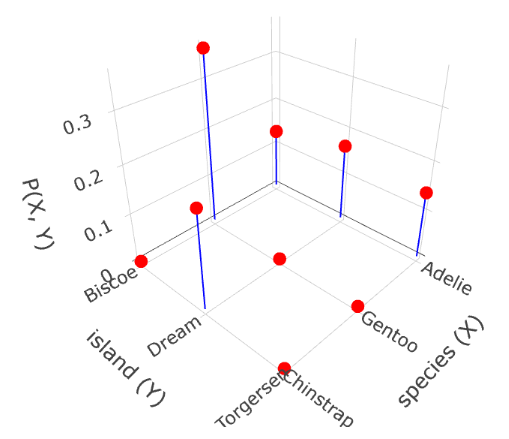
\includegraphics[width=0.7\linewidth]{SK_verzia_praca/figures/pravdeb_funk_ostrov_druhy_3D.png}
    \caption{3D znázornenie združenej pravdepodobnostnej funkcie (PMF) medzi premennými \textit{Ostrov ako miesto výskytu} a \textit{Druh} tučniakov.}
    \label{fig:miesto_druh_joint_density}
\end{figure}

Zatiaľ čo v jednorozmernom spojitom prípade nás zaujímala pravdepodobnosť výskytu náhodnej premennej v určitej oblasti na reálnej osi, v prípade dvoch spojitých premenných nás už zaujíma pravdepodobnosť, že realizácie oboch premenných spadnú do danej oblasti v rovine $\mathbb{R}^2$.

Ak $R_1 = [x_1, x_1 + dx_1]$ a $R_2 = [x_2, x_2 + dx_2]$ sú malé intervaly okolo bodu $(x_1, x_2)$, potom pravdepodobnosť, že náhodný vektor $(X_1, X_2)$ spadne do oblasti $R_1 \times R_2$, je približne:

\begin{equation}
\mathrm{Pr}(x_1 \leq X_1 \leq x_1 + dx_1,\ x_2 \leq X_2 \leq x_2 + dx_2) \approx f(x_1, x_2) \, dx_1 \, dx_2
\end{equation}

kde $f(x_1, x_2)$ je hodnota združenej hustoty pravdepodobnosti v bode $(x_1, x_2)$.

Presnejšie, pravdepodobnosť, že sa realizácie oboch premenných nachádzajú v oblasti $[a_1, b_1] \times [a_2, b_2]$, vypočítame pomocou dvojnásobného integrálu:

\begin{equation}
\mathrm{Pr}(a_1 \leq X_1 \leq b_1,\ a_2 \leq X_2 \leq b_2) = \int_{a_2}^{b_2} \int_{a_1}^{b_1} f(x_1, x_2) \, dx_1 \, dx_2
\end{equation}

Aby funkcia $f(x_1, x_2)$ bola platnou hustotou pravdepodobnosti, musí platiť:

\begin{equation}
\iint_{\mathbb{R}^2} f(x_1, x_2) \, dx_1 \, dx_2 = 1
\end{equation}

Združená hustota veľmi efektívne popisuje spoločné správanie sa dvoch spojitých náhodných premenných a tvorí základ pre ďalšie koncepty ako sú marginálne a podmienené rozdelenia.

Na nasledujúcom obrázku môžeme vidieť príklad vizualizácie združenej hustoty pravdepodobnosti homogénnej spojitej štruktúry dvoch premenných, pričom ako model výpočtu tu používame jadrové vyhladzovanie, viď ~\ref{textbf:kernel_smoothing}.

\begin{figure}[htpb]
    \centering
    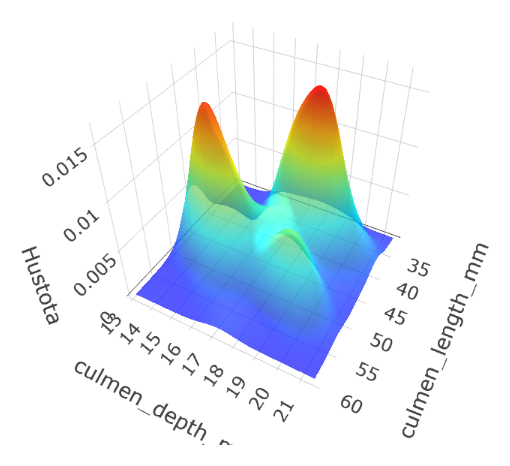
\includegraphics[width=0.7\linewidth]{hustota_hlbka_dlzka_zobaku_3D}
    \caption{3D znázornenie združenej hustoty pravdepodobnosti (PDF) medzi premennými \textit{Hĺbka zobáku} a \textit{Dĺžka zobáku} tučniakov.}
    \label{fig:zobak_joint_density}
\end{figure}

\subsection{Bodové charakteristiky}\label{joint_moments}

Rovnako ako v jednorozmernom prípade, aj v prípade viacrozmerných náhodných veličín (náhodného vektora) sú základnými charakteristikami rozdelenia \textit{stredná hodnota} a \textit{rozptyl}, pričom tentokrát si zavedieme aj pojem \textit{kovariancie}.

\subsubsection{Stredná hodnota}\label{subsubsec:joint_mean}

Pre náš dvojrozmerný náhodný vektor \(\vec{X} = (X_1, X_2)\) definujeme vektor stredných hodnôt ako:

\begin{equation}
\mathbb{E}[\vec{X}] = \left( \mathbb{E}[X_1], \mathbb{E}[X_2] \right)
\end{equation}

Pre obidva komponenty ho môžeme vyjadriť pomocou marginálnej hustoty (bližšie popísané v kapitole o marginálnom rozdelení~\ref{subsec:marginal_dist}). Napríklad pre \(X_1\) a marginálnu hustotu \(f_1(x_1)\) platí:

\begin{equation}
\mathbb{E}[X_1] = \int_{\mathbb{R}} x_1 \, f_1(x_1) \, dx_1
\end{equation}

alebo pomocou združenej hustoty:

\begin{equation}
\mathbb{E}[X_1] = \iint_{\mathbb{R}^2} x_1 \, f(x_1, x_2) \, dx_1 \, dx_2
\end{equation}

\subsubsection{Rozptyl}\label{subsubsec:joint_variance}

Rozptyl (disperzia) je definovaný ako očakávaná kvadratická odchýlka od strednej hodnoty:

\begin{equation}
\mathrm{Var}[X_1] = \mathbb{E}[(X_1 - \mathbb{E}[X_1])^2]
\end{equation}

Alternatívne možno rozptyl zapísať aj ako rozdiel momentov:

\begin{equation}
\mathrm{Var}[X_1] = \mathbb{E}[X_1^2] - (\mathbb{E}[X_1])^2
\end{equation}

\subsubsection{Kovariancia}\label{subsubsec:joint_covariance}

Kovariancia vyjadruje mieru lineárnej závislosti medzi dvoma náhodnými premennými \(X_1\) a \(X_2\). Definujeme ju ako:

\begin{equation}
\mathrm{Cov}[X_1, X_2] = \mathbb{E}[(X_1 - \mathbb{E}[X_1])(X_2 - \mathbb{E}[X_2])]
\end{equation}

Kovariancia sa dá alternatívne vyjadriť aj pomocou spoločného momentu:

\begin{equation}
\mathrm{Cov}[X_1, X_2] = \mathbb{E}[X_1 X_2] - \mathbb{E}[X_1] \cdot \mathbb{E}[X_2]
\end{equation}

Tieto hodnoty sa sumarizujú do dvojdimenzionálnej \textit{kovariančnej matice} \(\Sigma\), ktorá je symetrická a pozitívne semidefinitná:

\begin{equation}
\Sigma = 
\begin{bmatrix}
\mathrm{Var}[X_1] & \mathrm{Cov}[X_1, X_2] \\
\mathrm{Cov}[X_2, X_1] & \mathrm{Var}[X_2] \\
\end{bmatrix}
\end{equation}

Kovariančná matica je nevyhnutným nástrojom pre analýzu rozptylu a závislostí medzi komponentami náhodného vektora. Využíva sa napríklad pri odhade parametrov v lineárnej regresii alebo v diskriminačnej analýze.

\subsection{Marginálne rozdelenie}\label{subsec:marginal_dist}

Ak nás nezaujíma spoločné správanie všetkých náhodných premenných vektorovej premennej $\vec{X} = (X_1, X_2)$, ale iba jedného jej komponentu, môžeme skúmať jej vlastné pravdepodobnostné rozdelenie. Takéto rozdelenie nazývame \textit{marginálne rozdelenie} (angl. marginal distribution).

Na vizualizáciu marginálneho rozdelenia danej premennej, napríklad $X_2$, môžeme premietnuť každý bod z roviny $(x_1, x_2)$ na os $x_2$ a zostrojiť tak histogram týchto projekcií. Výsledný histogram, po normalizácii tak, aby plocha všetkých stĺpcov bola rovná 1, poskytuje empirický odhad marginálnej hustoty $f_2(x_2)$.

\begin{figure}[H] 
    \centering 
    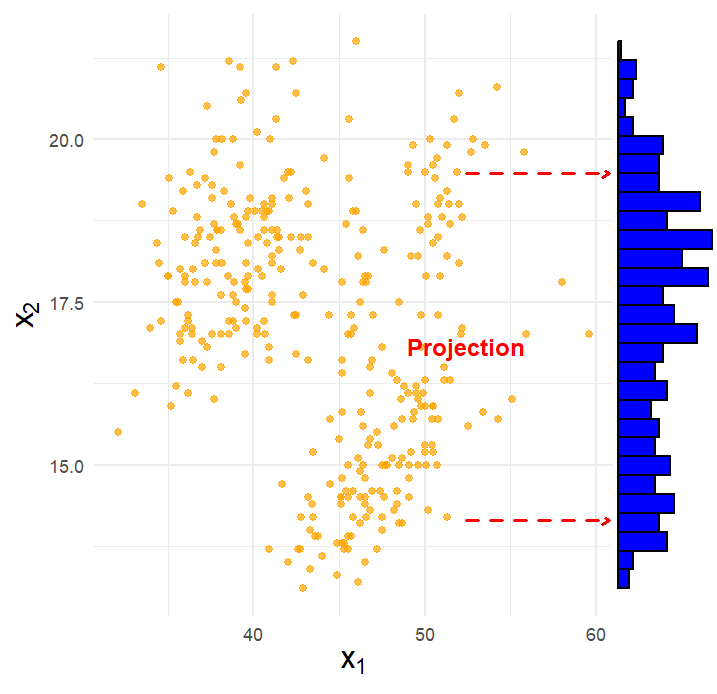
\includegraphics[width=0.7\linewidth]{marg_proj_hist.png} 
    \caption{Empirický odhad marginálneho rozdelenia $f_2(x_2)$} 
    \label{fig:margin_proj} 
\end{figure}

Z iného pohľadu, marginálne rozdelenie premennej $X_2$ vyjadruje pravdepodobnosť, že hodnota $X_2$ spadne do veľmi úzkeho intervalu $[x_2, x_2 + dx_2]$. V kontexte dvojrozmerného bodového grafu to zodpovedá pravdepodobnosti, že sa bod $(x_1, x_2)$ nachádza v horizontálnom páse výšky $dx_2$.

\begin{figure}[H]
    \centering
    \begin{subfigure}[b]{0.48\linewidth}
        \centering
        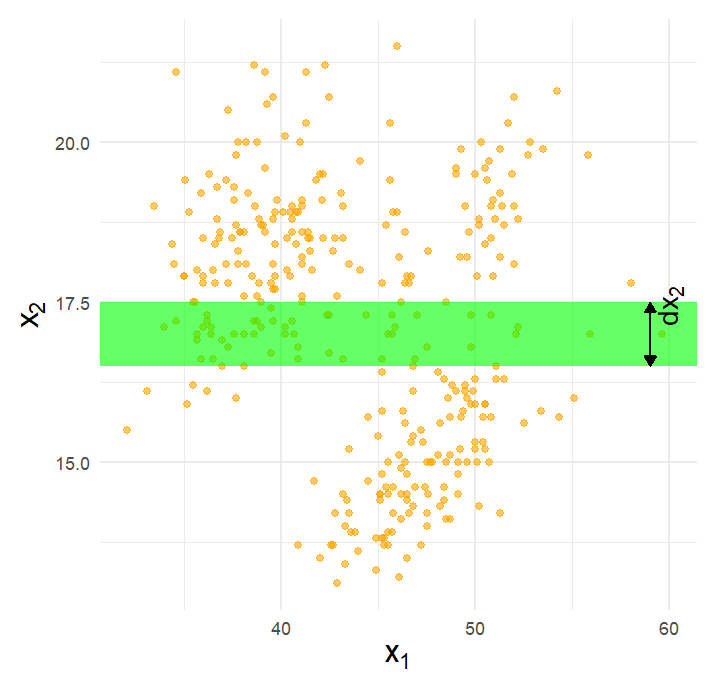
\includegraphics[width=\linewidth]{marg_strip_sum1.png}
        \caption{Horizontálny pás šírky $dx_2$ reprezentujúci interval pre $X_2$.}
        \label{fig:marg_strip_a}
    \end{subfigure}
    \hfill
    \begin{subfigure}[b]{0.48\linewidth}
        \centering
        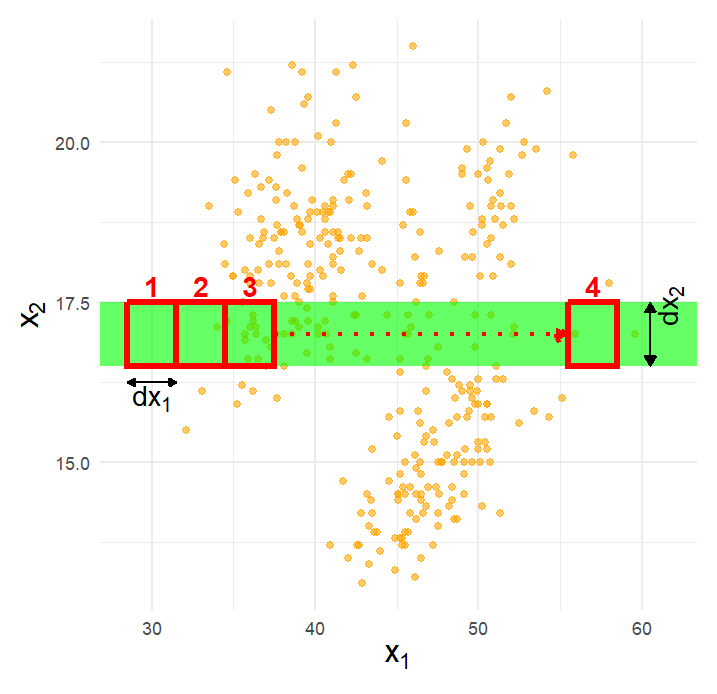
\includegraphics[width=\linewidth]{marg_strip_sum2.png}
        \caption{Pás rozdelený na plôšky $dx_1 \cdot dx_2$, z ktorých sa skladá marginálne rozdelenie $f_2(x_2)$.}
        \label{fig:marg_strip_b}
    \end{subfigure}
    \caption{Vizuálna interpretácia marginálneho rozdelenia $f_2(x_2)$}
    \label{fig:marg_strip}
\end{figure}

Ak si pás rozdelíme na plôšky $dx_1 \cdot dx_2$  (Obr.~\ref{fig:marg_strip_b}), potom z nich váženým súčtom dostaneme:

\begin{equation}
\mathrm{Pr}(x_2 \leq X_2 \leq x_2 + dx_2) \approx \sum_i f(x_1^{(i)}, x_2) \, dx_1 \, dx_2
\end{equation}

Porovnaním so vzťahom pre jednorozmernú hustotu pre spojité premenné nám vychádza vzťah, ktorý hovorí o tom, že marginálne rozdelenie $X_2$ možno získať z hustoty združeného rozdelenia $f(x_1, x_2)$ integráciou cez všetky hodnoty $x_1$:

\begin{equation} f_2(x_2) = \int_{-\infty}^{\infty} f(x_1, x_2) dx_1 \end{equation}

Podobne marginálne rozdelenie premennej $X_1$ získame ako:

\begin{equation} f_1(x_1) = \int_{-\infty}^{\infty} f(x_1, x_2)  dx_2 \end{equation}

Tieto marginálne rozdelenia slúžia ako základ pre rozklad združeného rozdelenia pomocou kopúl, ktorý bude predmetom nasledujúcej podkapitoly.

\begin{figure}[H]
    \centering
    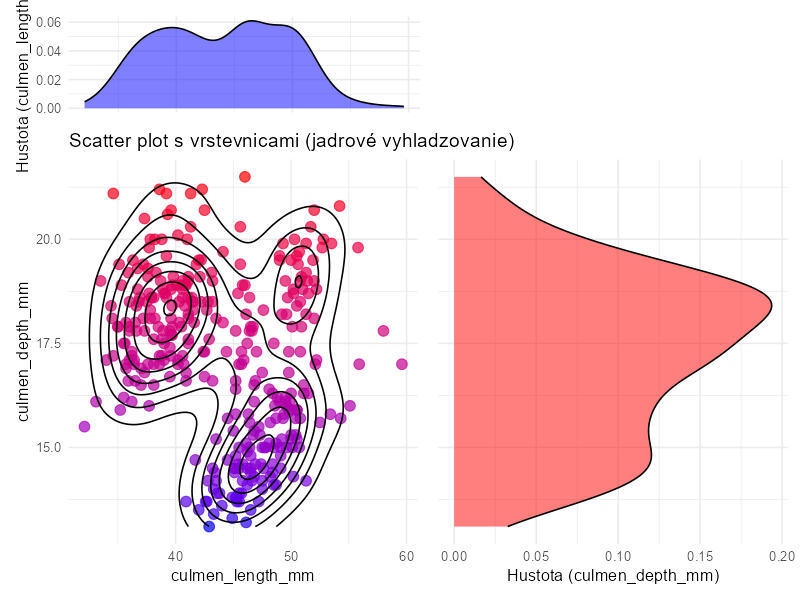
\includegraphics[width=0.8\linewidth]{hustota_hlbka_dlzka_zobaku_2D}
    \caption{Vrstevnice združenej PDF(Obr.~\ref{fig:zobak_joint_density}) + po bokoch marginálne PDF premenných \textit{Hĺbka zobáku} a \textit{Dĺžka zobáku} tučniakov (metóda: jadrové vyhladzovanie ~\ref{textbf:kernel_smoothing})}
    \label{fig:zobak_marg_density}
\end{figure}

\subsection{Podmienené rozdelenie}\label{subsec:conditional_distribution}

Kým marginálne rozdelenie opisuje správanie jednej premennej bez toho aby sa bral do úvahy vplyv ostatných premenných na túto premennú, v mnohých praktických situáciách nás zaujíma, ako sa rozdelenie jednej premennej mení v závislosti od známych hodnôt inej premennej. V takýchto prípadoch hovoríme o \textit{podmienenom rozdelení}.

\subsubsection{Hustota}\label{subsubsec:conditional_density}

Formálne, ak máme náhodný vektor $(X_1, X_2)$, potom podmienená hustota premennej $X_2$ vzhľadom na známu hodnotu $X_1 = x_1$ je definovaná ako:

\begin{equation}
f_{2 \mid 1}(x_2 \mid x_1) = \frac{f(x_1, x_2)}{f_1(x_1)},
\end{equation}

kde:
\begin{itemize}
  \item $f(x_1, x_2)$ je združená hustota,
  \item $f_1(x_1) = \int_{-\infty}^{\infty} f(x_1, x_2) \, dx_2$ je marginálna hustota premennej $X_1$.
\end{itemize}

Z definície o podmienenej pravdepodobnosti vyplýva:

\begin{equation}
\mathrm{Pr}(a \leq X_2 \leq b \mid X_1 = x_1) = \int_a^b f_{2 \mid 1}(x_2 \mid x_1) \, dx_2.
\end{equation}

Podmienenú hustotu tu taktiež možno intuitívne interpretovať ako hustotu v rámci tenkého vertikálneho pásu, kde náhodná premenná $X_1$ nadobúda hodnoty z intervalu $[x, x + \varepsilon]$ (Obr.~\ref{fig:cond_density_strip}). V tomto pásme vyberieme všetky body, ktoré spadajú do intervalu $[x, x + \varepsilon]$, a z nich vytvoríme histogram hodnôt premennej $X_2$, čím získame empirický odhad hustoty $f_{2 \mid 1}(x_2 \mid X_1 = x)$.

Tento postup je znázornený na nasledujúcom obrázku:

\begin{figure}[H]
    \centering
    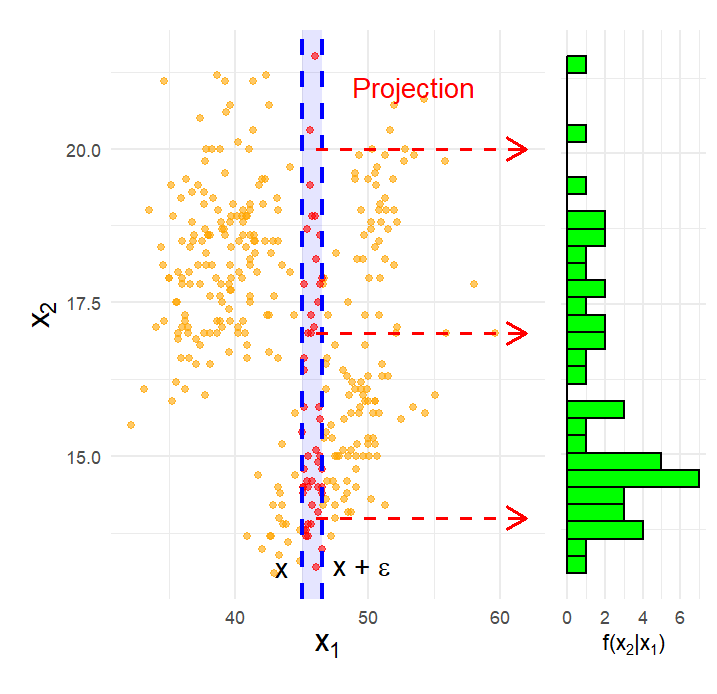
\includegraphics[width=0.7\linewidth]{marg_condition_strip.png}
    \caption{Empirický odhad podmienenej hustoty $f_{2 \mid 1}(x_2 \mid x_1 \in [x, x + \epsilon])$}
    \label{fig:cond_density_strip}
\end{figure}

Týmto sme zaviedli pojem podmienenej hustoty, ktorý bude ďalej kľúčový pri výpočte tzv. \textit{podmienenej strednej hodnoty}.

\subsubsection{Podmienená stredná hodnota}\label{subsubsec:conditional_mean}

\section{Rozklad}\label{sec:rozklad_kopule}
\section{Odhad}\label{sec:odhad}